\chapter{Case Study - Knowledge Graphs}

A Knowledge Graph (KG), represents a collection of interlinked descriptions of entities - real-world objects, events, situations or abstract concepts. The entities are represented as nodes and the relationships between them as edges. The nodes and edges are labeled with attributes that describe the entities and relationships.

Just like any Graph, the KG is made up of nodes and edges, where the edges have a direction, indicating the direction of the relationship between a pair of concepts.

A KG is a structured representation of knowledge, which can be used understood as a `Graph of Concepts', to infer new knowledge, answer questions, and discover new relationships between entities. It is a powerful tool for representing and reasoning about complex relationships between entities in a domain.

\section{Knowledge Graphs in the Real World}

Knowledge Graphs are used in a variety of applications.
Any text corpus can be visualised in an interactive and intuitive
manner.

Graph Databases like Neo4j\cite{n4j}, Amazon Neptune\cite{neptune}, and JanusGraph\cite{janus} are a way to store and query data in the form of a graph. They are used in a variety of applications, including social networks, recommendation systems, fraud detection, and network analysis.

\section{Creating Knowledge Graphs using LLMs}

Large Language Models (LLMs) like GPT-3.5\cite{gpt3} and BERT\cite{bert} can be used to create Knowledge Graphs from unstructured text.
Through the use of fine-tuning and prompt engineering on a specific domain or dataset these models can be used to generate a KG from the text.

\subsection{Our Approach}

We use the Google's generative AI suite to access the `Gemini-1.0-pro' model to generate a
a structured representation of Knowledge Graph from a text corpus through a user given prompt or a
an already existing text corpus.

We use create tools to implement generation of KGs through function calling and
provide a user-friendly interface to interact with the model.


\subsection*{Examples}

Consider the following verse taken from the Hollow Knight game:\vspace*{1em}

\makeatletter
\renewcommand{\@chapapp}{}% Not necessary...
\newenvironment{chapquote}[2][2em]
{\setlength{\@tempdima}{#1}%
    \def\chapquote@author{#2}%
    \parshape 1 \@tempdima \dimexpr\textwidth-2\@tempdima\relax%
    \itshape}
{\par\normalfont\hfill--\ \chapquote@author\hspace*{\@tempdima}\par\bigskip}
\makeatother

\begin{chapquote}{\textit{The Pale King}}
    \noindent No cost too great.\\
    No mind to think.\\
    No will to break.\\
    No voice to cry suffering, \\[1em]
    Born of God and Void.\\
    You shall seal the blinding light that plagues their dreams.\\
    You are the Vessel.\\
    You are the Hollow Knight.
\end{chapquote}

This entire text can be converted into a Knowledge Graph, which can be used to
infer new knowledge, and discover new relationships between entities.

\pagebreak
\begin{figure}[h!]
    \centering
    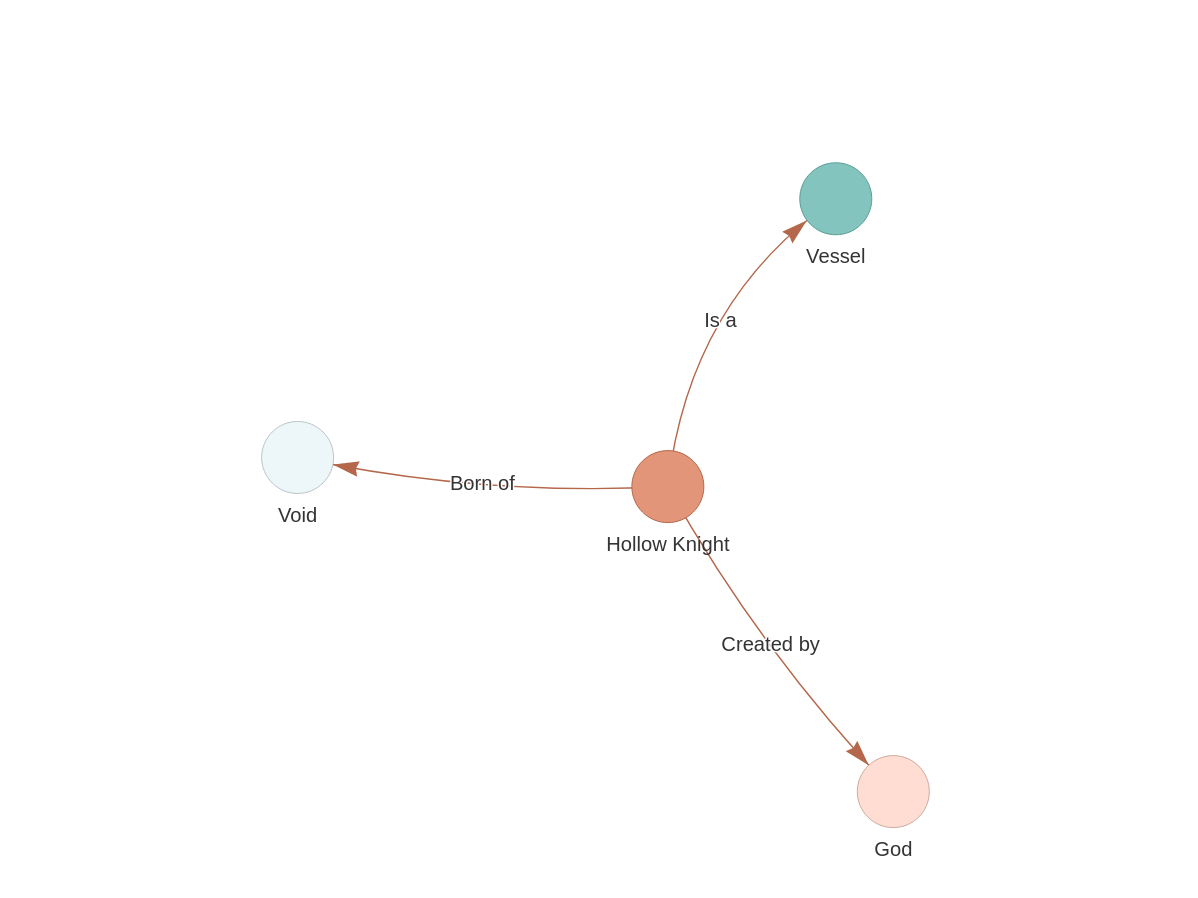
\includegraphics[width=0.9\textwidth]{images/hknobg.png}
    \caption{Corpus based Knowledge Graph}
    \label{fig:hk}
\end{figure}


Our approach\cite{korigamikkg} can also
create the following Knowledge Graph based on a user prompt:

\begin{verbatim}
User Prompt: "How does the Transformer model work?"
\end{verbatim}

Which generates the following Knowledge Graph:

\begin{verbatim}
Knowledge Graph:
{
    "name": "add_to_database",
    "args": {
        "entities": [
            {
                "description": "Neural network model for natural 
                language processing tasks",
                "type": "Model",
                "name": "Transformer Model Architecture"
            },
            ...
        ],
        "relationships": [
            {
                "to_entity_name": "Encoder",
                "relationship": "Composed of",
                "from_entity_name": "Transformer Model Architecture"
            },
            ...
        ]
    }
}

\end{verbatim}


The generated Knowledge Graph represents the relationships between the entities in the text, and can be used to answer questions, infer new knowledge, and discover new relationships between entities.

\begin{figure}[h!]
    \centering
    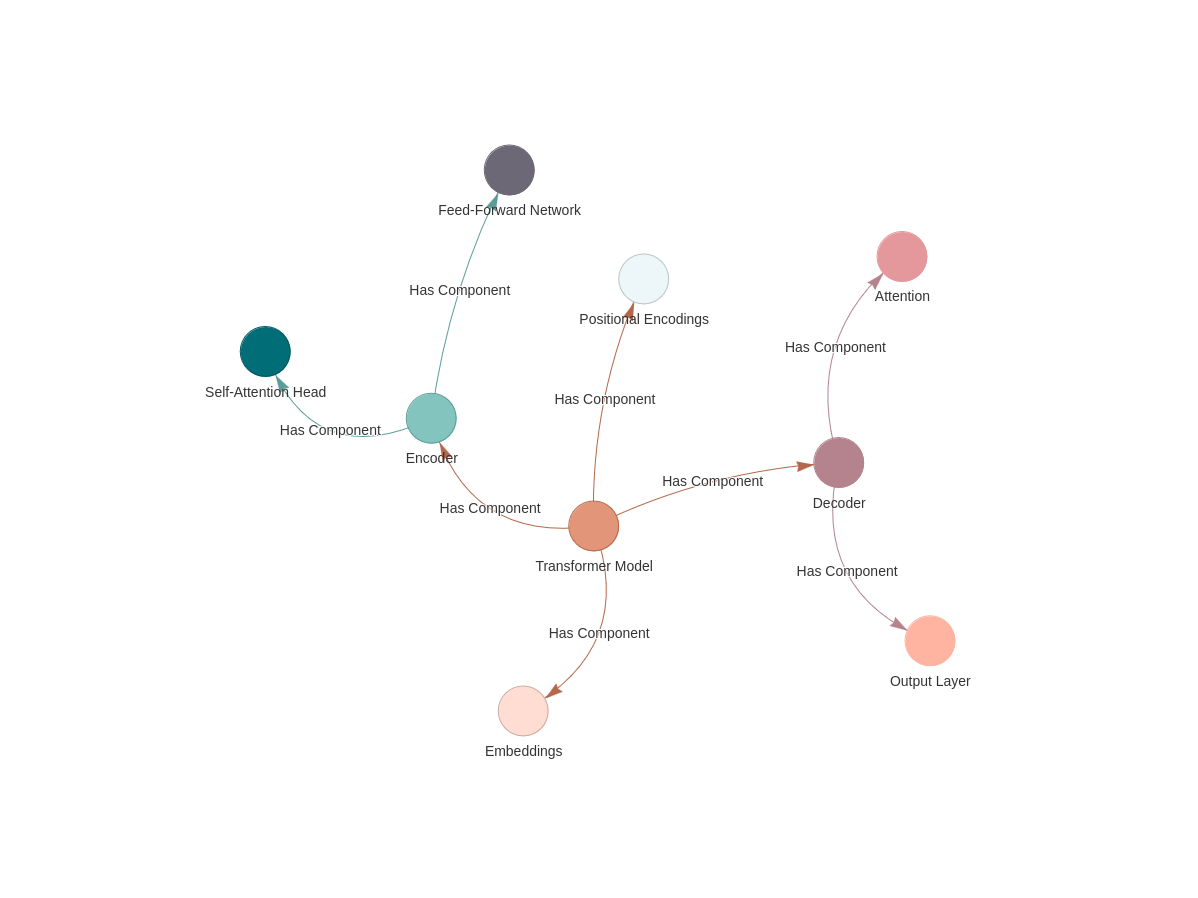
\includegraphics[width=0.9\textwidth]{images/transformer.png}
    \caption{Prompted Knowledge Graph: Transformer}
    \label{fig:kg}
\end{figure}

\section{Applications}

Knowledge Graphs have been used in  a slew of different industries and applications. These are used by researchers, marketing professionals, and data scientists to understand the relationships between entities in a domain, and to infer new knowledge from the data.

Recommendation systems and search engines use Knowledge Graphs to provide more relevant and accurate results to users. They can be used to answer questions, infer new knowledge, and discover new relationships between entities in a domain.

Inspite of these large scale applications, KGs can be used in a more personal and individual level. They can be used to create a personal knowledge base, to store and organize information, and to help you remember and recall information more easily.
They allow us to understand concepts at a glance and can be used to create a visual representation of a text corpus.

